\subsection{Tools for working with ngs alignments}

\begin{frame}
\frametitle{Samtools}
\begin{center}
\begin{itemize}
\item
Program to work with ngs alignment files (SAM, BAM, CRAM)
\item
Can be used to view data, calculate basic info, extract subsets of alignments and convert between file formats
\item
http://www.htslib.org
\end{itemize}
\end{center}
\end{frame}

\begin{frame}
\frametitle{Picard}
\begin{center}
\begin{itemize}
\item
A set of Java command line tools with the same (or similar functionality as samtools)
\item
Note that even though they largely aim at doing similar functions Picard and Samtools is not always generating compatible file formats
\item
http://broadinstitute.github.io/picard/
\end{itemize}
\end{center}
\end{frame}

\begin{frame}{Samtools tview, a text-based alignment viewer}
\begin{center}
\$ samtools view alignment.bam target.fasta\\
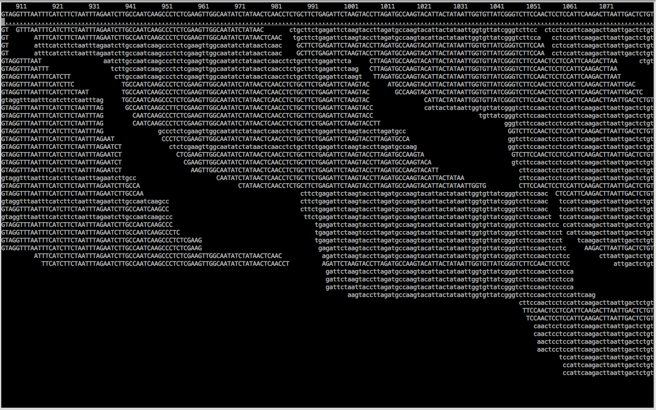
\includegraphics[width=10cm]{Images/tview.png}
\end{center}
\end{frame}

\begin{frame}{IGV: Integrative Genomics Viewer}
\begin{center}
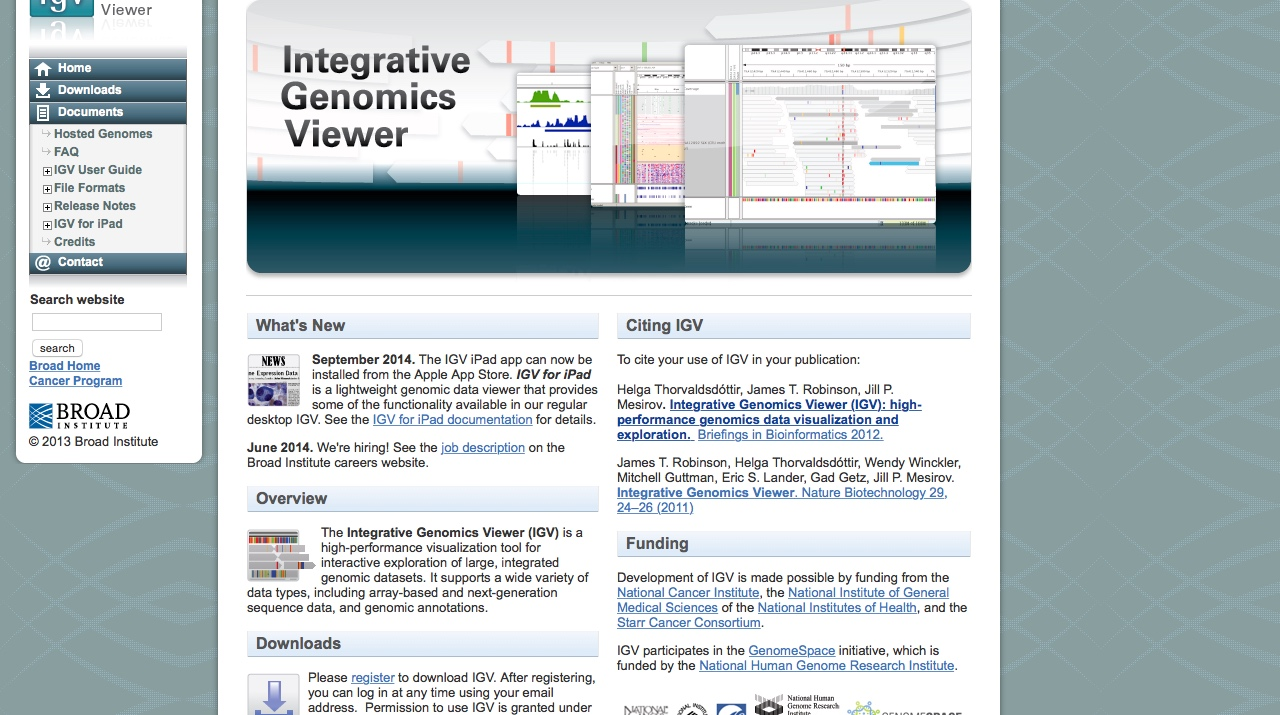
\includegraphics[width=10cm]{Images/IGV.jpg}
\end{center}
\end{frame}

\begin{frame}{IGV: Integrative Genomics Viewer}
\begin{center}
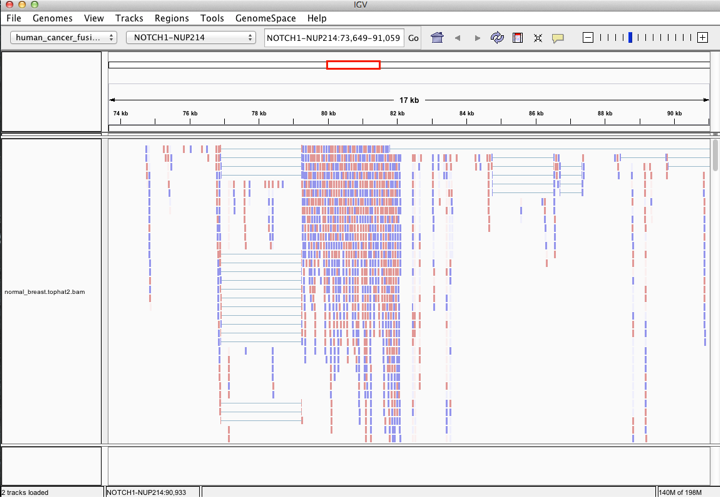
\includegraphics[width=10cm]{Images/IGValign.png}
\end{center}
\end{frame}
